\icode{E-MI-MU-L3-261106-001}
（多选）
在粗糙水平面上静置一个质量为\(M\)的三角形斜劈\(A\)(两侧斜面倾角不相等，满足\(\alpha > \beta\))，此时两个质量均为\(m\)的小物块\(P\)和\(Q\)恰沿两侧斜面匀速下滑。若在下滑过程中，同时各施加一个平行于各自斜面的大小相等的恒力\(F_1\)、\(F_2\)作用于两物块，如图所示，重力加速度为\(g\)，则在施	力后\(P\)和\(Q\)下滑过程中（均未到达底端），下列判断正确的是\paren[]

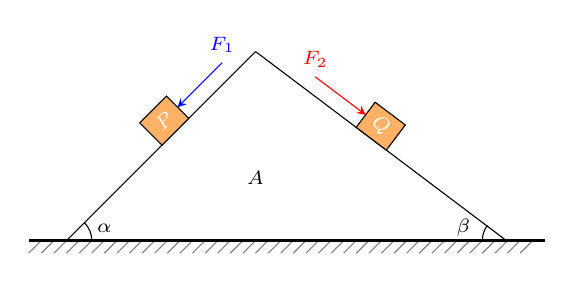
\begin{tikzpicture}[scale=.8,>=stealth,font=\scriptsize]
	\begin{scope}[rotate=-37]
		\draw (0,0)--(5,0);
		\draw[fill=orange!60] (2,0) rectangle(2.6,.5)node[white,midway,rotate=-30]{\(Q\)};
		\draw[->,red] (1,.25)node[above]{\(F_2\)}--(2,.25);
	\end{scope}
	\begin{scope}[rotate=45]
		\draw(0,0)--({-3*sqrt(2)},0);
		\draw[fill=orange!60] (-1.5,0)rectangle(-2.1,.5)node[white,midway,rotate=45]{\(P\)};
		\draw[->,blue] (-.5,.25)node[above]{\(F_1\)}--(-1.5,.25);
	\end{scope}
	\draw (-135:{3*sqrt(2)})--(-37:5);
	\draw[xshift=-3cm,yshift=-3cm] (.4,0) arc(0:45:.4);
	\draw[xshift=4cm,yshift=-3cm] (-.4,0) arc(180:143:.4);
	\foreach \x in {-3.6,-3.4,...,4.4}
	    \draw[gray] (\x,-3.2)--++(.2,.2);
	\draw[thick] (-3.6,-3)--(4.6,-3);
	\node at(-2.4,-2.8){\(\alpha\)};
	\node at(3.3,-2.8){\(\beta\)};
	\node at(0,-2){\(A\)};
\end{tikzpicture}
\begin{choices}
	\item 物块\(P\)和物块\(Q\)的加速度大小相等
	\item 地面对斜劈\(A\)的支持力大小为\((M+2m)g\)
	\item 斜劈\(A\)有向右的运动趋势
	\item 若将\(F_2\)的方向改为竖直向下，地面与斜劈\(A\)之间没有摩擦力
\end{choices}
\begin{answer}
	ABD\qquad 提示：
\end{answer}